%-----------------------------------------------------------------------------%
\chapter{\babDua}
%\begin{center}
%	\textbf{BAB II}
%	\par \textbf{TINJAUAN PUSTAKA}
%\end{center}
%---------------------------------------------------------------------------%-----------------------------------------------------------------------------%
%  \section{\textit{Visible Light Communication}}
 
%  \textit{Visible Light Communication} (VLC) merupakan teknologi komunikasi yang memanfaatkan sumber cahaya dengan gelombang tampak sebagai \textit{transmitter}, udara sebagai media transmisi, dan \textit{photodetector} sebagai \textit{receiver}....
% \par 
  
%  \section{\textit{Light Emitting Diode}}
 
%  \textit{Light Emitting Diode} (LED) adalah....
 
% \begin{figure}
% 	\centering
% 	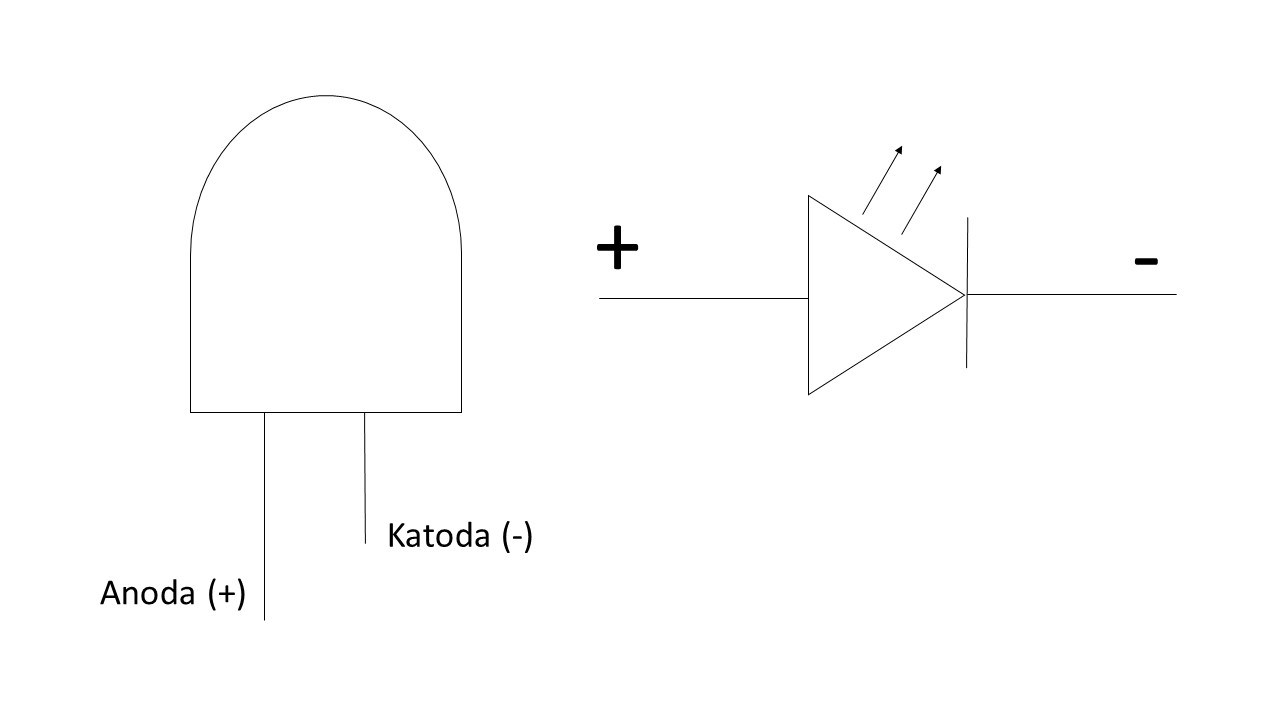
\includegraphics[width=0.6\linewidth]{pics/led}
% 	\caption{\textit{Light emitting diode}.}
% 	\label{fig:led}
% \end{figure}
 
% \section{\textit{Photodetector}}
% \textit{Photodetector} menggunakan fotodioda.....	
% \par


% \section{\textit{Line of Sight}}
% Pada VLC terdapat dua jenis kanal yang terapkan dalam saluran transmisi optik yaitu \textit{Line of Sight} (LOS) dan \textit{Non-Line of Sight} (NLOS)....
% \begin{figure}
% 	\centering
% 	\includegraphics[width=0.4\linewidth]{"pics/TANat/ilustrasi kanal los"}
% 	\caption{Ilustrasi kanal LOS.}
% 	\label{fig:ilustrasi-kanal-los}
% \end{figure}
% Model kanal LOS direpresentasikan pada Gambar \ref{fig:ilustrasi-kanal-los}. Simbol h adalah tinggi \textit{transmitter}, d adalah jarak antara \textit{transmitter} dan \textit{receiver}, dan $\phi$ adalah sudut yang dibentuk antara \textit{transmitter} dan \textit{receiver}.
% \par
% Distribusi sudut dari pola intensitas radiasi dimodelkan menggunakan intensitas lambertian umum yang dinyatakan dengan
% \begin{equation}
% \label {lambertian}
% m=\frac{-\ln 2}{\ln \left(\cos \Phi _{1/2}\right)},
% \end{equation}
% dengan $m$ adalah persamaan lambertian dan $\phi_{1/2}$ adalah nilai \textit{full width at half maximum}.

% Pengiriman data dari \textit{transmitter} ke \textit{receiver} menggunakan kanal \textit{indoor} LOS pada \textit{Optical Wireless Communication} (OWC) yang dapat dirumuskan sebagai berikut \cite{ghassemlooy2013indoor}
% \begin{equation}
% \label{kanal}
% H=\frac{\left(m+1\right)\cdot A_{det}\cdot \cos ^{\left(m+1\right)}\left(\Phi \right)}{2\cdot \pi \cdot d^2},
% \end{equation}
% dengan $A_{det}$ yaitu area \textit{photodetector} di sisi penerima, $d$ merupakan jarak penerima terhadap sisi pengirim, dan $\Phi$ adalah sudut perpindahan terhadap \textit{transmitter}.